%!TEX program = pdflatex
\documentclass[12pt,a4paper]{article}

% ---- Typography & Design ----
\usepackage[utf8]{inputenc}
\usepackage[T1]{fontenc}
\usepackage[protrusion=true, expansion=false]{microtype}  % better character protrusion
\usepackage[margin=1in, bottom=1.1in]{geometry} % slightly taller text block
\usepackage{setspace}
\usepackage{parskip}                            % skip between paragraphs, no indent
    \setlength{\parskip}{4pt plus 1pt minus 1pt}
\usepackage{fancyhdr}                           % running headers
\usepackage{titlesec}                           % custom section formatting
\usepackage[labelfont=bf,font=small]{caption}
\usepackage[labelfont=bf,font=footnotesize]{subcaption}
\usepackage{float}
\usepackage{enumitem}
\usepackage{array}
\usepackage{xcolor}
\usepackage[colorlinks=true, linkcolor=blue!60!black, citecolor=blue!60!black, urlcolor=blue!60!black]{hyperref}

% ---- Math ----
\usepackage{amsmath,amssymb,amsfonts}
\usepackage{tikz}
\usetikzlibrary{arrows,shapes.geometric,positioning,fit,backgrounds,decorations.pathreplacing,calc}
\usepackage{graphicx}
\usepackage{booktabs}

\onehalfspacing

% ---- Section formatting ----
\titleformat{\section}{\Large\bfseries}{\thesection}{1em}{}
\titleformat{\subsection}{\large\bfseries}{\thesubsection}{1em}{}
\titleformat{\subsubsection}{\normalsize\bfseries}{\thesubsubsection}{1em}{}

% ---- Running headers ----
\setlength{\headheight}{14.5pt}
\pagestyle{fancy}
\fancyhf{}
\fancyhead[L]{\small\itshape Probabilistic Demand Forecasting During Extreme Winter Events}
\fancyhead[R]{\small\thepage}
\renewcommand{\headrulewidth}{0.4pt}

% ---- Commands ----
\newcommand{\R}{\mathbb{R}}
\newcommand{\E}{\mathbb{E}}


\titlespacing*{\section}{0pt}{18pt plus 4pt minus 2pt}{10pt plus 2pt minus 2pt}
\titlespacing*{\subsection}{0pt}{14pt plus 3pt minus 2pt}{8pt plus 2pt minus 1pt}
\begin{document}

\title{\LARGE\textbf{Probabilistic Electricity Demand Forecasting During Extreme Winter Events: A Case Study of the 2014 Polar Vortex in PJM}}
\author{Dresden E. Goehner\\[4pt]
\textit{Independent Researcher}}
\date{}
\maketitle

\begin{abstract}
Accurate short-term load forecasting during extreme cold-weather events is critical for grid reliability, yet standard probabilistic evaluation frameworks aggregate performance across all operating conditions and may conceal systematic undercoverage precisely when grid stress is highest. This study evaluates gradient boosted quantile regression (QR-GBT) on the January 6–8, 2014 PJM Polar Vortex --- a near-annual-peak cold-weather stress event in which RTO load reached 140,510.2 MW --- using PJM hourly load data from 2010 through 2014 and same-hour ERA5 retrospective reanalysis weather inputs, which provide an idealized retrospective weather-information setting rather than an operational forecast-weather setting.

 On point accuracy, a gradient boosted model achieves a full-year mean absolute error of 721 MW against a PJM Day-Ahead benchmark of 1,937 MW; during the vortex window the same model records 1,705 MW MAE against 3,148 MW for the Day-Ahead benchmark, with both comparisons reflecting the ERA5 retrospective setting rather than operational superiority. Despite 86.8\% empirical coverage at the nominal 90\% prediction interval level across full-year 2014 evaluation, QR-GBT coverage collapses to 66.7\% during the 72-hour vortex window, 98\% interval coverage falls to 84.7\%, and the observed load exceeds the post-rearrangement q99 estimate of 139,585 MW, leaving the event peak outside the nominal 98\% prediction interval. These results demonstrate that full-year calibration metrics can mask severe tail undercoverage under distribution-shifting cold-weather stress, and that disaggregated evaluation on historical extreme windows is a necessary complement to annual probabilistic benchmarking.
\end{abstract}

\newpage\tableofcontents\newpage

\section{Introduction}
\subsection{Load Forecasting and Grid Reliability}
Reliable short-term load forecasting is foundational to the secure and economical operation of bulk electric power systems. System operators depend on accurate hourly demand forecasts to schedule generating units, procure operating reserves, clear day-ahead energy markets, and manage transmission constraints \cite{hong2016tutorial}. When forecasts underestimate demand --- particularly at system peaks --- the consequences are immediate: reserve margins erode, emergency procedures may be triggered, and real-time prices can spike sharply as operators scramble to secure additional capacity \cite{nerc2014polar,pjm2014polar}. Conversely, systematic overestimation wastes reserve capacity and increases costs for consumers. The stakes are not symmetric: in a high-load emergency, a forecasting error of several gigawatts can be the difference between controlled load management and an uncontrolled reliability event. This operational asymmetry motivates particular attention to the accuracy of forecasts during extreme demand periods.


\subsection{Probabilistic Forecasting and Prediction Intervals}
Point forecasts --- single-valued predictions of expected demand --- have long been the operational standard, but they provide no direct information about uncertainty. A point forecast of 130,000 MW carries the same face value whether the forecaster is highly confident or deeply uncertain. Probabilistic load forecasting addresses this by estimating the full conditional distribution of future demand, typically expressed as quantile forecasts or prediction intervals \cite{hong2016probabilistic}. Prediction intervals support a range of reliability-critical decisions that point forecasts cannot: procuring reserves calibrated to the tail of the demand distribution, setting offer caps in capacity markets, and communicating forecast uncertainty to transmission planners \cite{hong2016tutorial}. 

Despite these advantages, probabilistic forecasting methods are less uniformly adopted in operational practice than their deterministic counterparts, and the evaluation frameworks used to benchmark them --- typically aggregate annual metrics such as the Continuous Ranked Probability Score (CRPS) or empirical prediction interval coverage --- may not capture the behavior that matters most for grid reliability: performance during the small fraction of hours when load is at or near its annual extreme.
\subsection{Extreme Cold as a Tail-Risk Forecasting Problem}
Extreme cold-weather events present a qualitatively distinct forecasting challenge. In large interconnections with significant heating load, cold air outbreaks drive demand responses that differ materially from the moderate-winter conditions that dominate any multi-year training dataset. The load-temperature relationship is nonlinear: each additional degree of cold below the heating base temperature drives progressively larger demand increases as less-efficient heating systems engage and as behavioral responses compound meteorological forcing \cite{fan2012shortterm}. A data-driven forecasting model trained primarily on moderate winters will have seen few or no examples of the load levels that arise during a severe cold air outbreak, placing the event in or near the extrapolation regime of the model's learned input-output mapping. 

Under these conditions, a model may produce point forecasts with acceptable average error while simultaneously constructing prediction intervals that are far too narrow --- assigning insufficient probability mass to the load levels that actually occur at the peak hour. This distinction between average-case and tail-case probabilistic performance is directly observable in the present case study: QR-GBT achieves 86.8\% full-year 90\% PI coverage but only 66.7\% during the vortex window, highlighting the value of evaluating probabilistic forecasters on disaggregated extreme-event windows rather than relying solely on full-year aggregate calibration diagnostics.
\subsection{The January 2014 PJM Polar Vortex as a Case Study}
The January 2014 polar vortex provides a well-documented and historically significant test of load forecasting under extreme cold stress. The January 6–8, 2014 Polar Vortex produced a near-annual-peak RTO load of 140,510.2 MW at Jan 7 18:00 EPT, equal to 99.18\% of the 2014 annual peak of 141,677.9 MW recorded on Jun 17 17:00 EPT. This event was the subject of detailed post-event reviews by both NERC and PJM, which documented widespread generation unit failures, emergency energy transactions, and significant forecast errors by multiple market participants \cite{nerc2014polar,pjm2014polar}. Several factors make this event particularly suited to a rigorous retrospective forecasting study.

 First, the event load is near the 2014 annual system peak, making it a genuine extreme in the demand distribution rather than a moderate stress event. Second, complete, publicly accessible hourly load data from PJM Data Miner 2 and ERA5 retrospective reanalysis weather data from the Copernicus Climate Data Store are available for exact replication of the analysis. Third, the event occurred only one year into the evaluation period, meaning a model trained through 2013 had no exposure to a comparable cold air outbreak during training --- creating a clean test of out-of-distribution generalization. 

Fourth, the meteorological character of the event is well-characterized in the atmospheric science literature \cite{arritt2014us}, providing context for the thermodynamic forcing that drove the load response.
\subsection{This Study: What Is Evaluated and What Is Found}
This study evaluates a gradient boosted quantile regression model (QR-GBT) trained on 2010–2013 PJM hourly load data with ERA5 retrospective reanalysis weather features, assessed against two evaluation windows: full-year 2014 and the 72-hour January 6–8 polar vortex window. 

All weather-informed model results use same-hour ERA5 retrospective reanalysis weather input --- that is, the actual meteorological conditions as reconstructed by the ERA5 reanalysis system rather than a real-time operational weather forecast. This design tests whether a well-specified probabilistic model can adequately characterize demand uncertainty even under an idealized weather-knowledge setting; it does not simulate operational deployment. On point accuracy, the gradient boosted model substantially outperforms persistence and seasonal naive baselines across the full evaluation year and during the vortex window, with a full-year MAE of 721 MW compared to 1,937 MW for the PJM Day-Ahead benchmark (both comparisons in the retrospective ERA5 setting). 

However, the central finding is not the point forecast improvement but the probabilistic failure: despite 86.8\% empirical coverage at the 90\% nominal prediction interval level over the full year, QR-GBT coverage falls to 66.7\% during the vortex window, 98\% interval coverage falls to 84.7\%, and at the peak hour, the observed load exceeded the post-rearrangement QR-GBT q99 estimate of 139,585 MW, leaving the event peak outside the nominal 98\% prediction interval. The 19.8-percentage-point gap between full-year and vortex-window coverage at the 90\% level is invisible to any evaluation framework reporting only annual aggregate metrics --- and it is this gap, rather than the point forecast comparison, that is the paper's primary empirical contribution.
\subsection{Contributions and Organization}
This paper makes three contributions:

\begin{enumerate}
    \item We provide a retrospective evaluation of QR-GBT during the January 6–8, 2014 PJM Polar Vortex, demonstrating that a model achieving 86.8\% full-year empirical PI coverage nonetheless fails to cover the event peak of 140,510.2 MW at the nominal 98\% level, with the observed load exceeding the post-rearrangement q99 estimate of 139,585 MW. All results use same-hour ERA5 retrospective reanalysis weather input. This constitutes a quantified, documented case of probabilistic calibration failure under out-of-distribution extreme cold.
\item We show that the 19.8-percentage-point gap between full-year and vortex-window empirical coverage at the 90\% level is invisible to any evaluation protocol reporting only annual aggregate metrics, and that calibration degrades systematically across the high-load tail of the demand distribution. These findings argue for disaggregated evaluation on historical extreme windows as a necessary component of probabilistic load forecasting benchmarks in reliability-critical applications.
\item Using publicly available PJM Data Miner 2 load records and ERA5 reanalysis weather inputs, we construct a transparent retrospective benchmark on a historically significant event against which future extreme-event probabilistic forecasting methods can be compared, with all data sources, model specifications, and evaluation windows stated explicitly.
\end{enumerate}

The remainder of this paper is organized as follows. Section 2 describes the PJM load dataset, ERA5 weather inputs, preprocessing procedure, and the definition of the polar vortex case study window. Section 3 presents the quantile regression forecasting framework, model architecture, feature set, and benchmark models. Section 4 describes the experimental design and evaluation protocol. Section 5 reports results across both evaluation windows. Section 6 discusses the mechanisms underlying calibration failure and their implications for probabilistic forecasting evaluation practice. Section 7 states the study's limitations. Section 8 concludes.

\section{Data and Event Definition}
\subsection{PJM Load Data}
Hourly electricity demand data were obtained from PJM Data Miner 2 (Hourly Load: Metered), the publicly accessible load reporting portal maintained by PJM Interconnection. All records use RTO-level aggregate load, representing the metered demand across the full PJM transmission system. The analysis period spans January 1, 2010 through December 31, 2014, yielding 43,824 hourly observations prior to feature construction. Following the creation of lagged and rolling-window features with a maximum lookback of 168 hours, the first 168 observations are dropped to avoid partially undefined feature rows, leaving 43,656 complete observations available for modeling.


The dataset is partitioned into a training set covering January 1, 2010 through December 31, 2013 (34,896 observations) and a held-out test set covering the full calendar year 2014 (8,760 observations). Model fitting and feature construction use only information available within the training period; no 2014 observations are included in training. The 2014 test year is used solely for evaluation.


Table 1 summarizes the load distribution across the training period, the 2014 test year, and the two event comparison windows analyzed in this study. The training set spans a wider load range (49,558–158,043 MW) than the 2014 test year (57,570–141,678 MW). The gap between the training maximum (158,043 MW) and the 2014 test maximum (141,678 MW) is noted as distributional context; the causes of this difference are not analyzed in this study. Within this context, the 2014 near-peak cold-event load of 140,510 MW, while near the 2014 annual peak, is not near the upper boundary of the training load distribution.

\subsection{ERA5 Retrospective Weather Inputs}
Meteorological inputs are drawn from the ERA5 reanalysis dataset produced by the European Centre for Medium-Range Weather Forecasts (ECMWF) and distributed through the Copernicus Climate Data Store \cite{hersbach2020era5}. ERA5 provides hourly estimates of atmospheric variables on a global grid with approximately 31 km horizontal resolution, reconstructed through a numerical weather prediction model constrained by historical observations.
Three ERA5 near-surface variables are used: 2-metre air temperature (t2m), 10-metre zonal wind component (u10), and 10-metre meridional wind component (v10). Dewpoint temperature (d2m) was not included in the downloaded ERA5 files and is not used in the final modeling table.
Spatial aggregation uses the great\_lakes\_core subset, defined as a rectangular ERA5 grid box spanning 40.0°N–42.5°N and -88.0°W to -74.0°W at 0.25° resolution. The subset contains 627 grid cells, and each ERA5 variable is aggregated by a simple unweighted arithmetic mean over latitude and longitude. No population weighting is applied.
From these aggregated fields, derived features are constructed as follows. Temperature is converted from Kelvin to Fahrenheit. Wind speed is computed as sqrt(u10² + v10²) and converted from m/s to mph. Wind chill is computed using the NOAA/NWS wind chill formula when T $\leq$ 50$^\circ$F and wind speed exceeds 3 mph; otherwise wind chill is set equal to temperature. Heating and cooling degree hours are computed as HDH = max(65 - T$^\circ$F, 0) and CDH = max(T$^\circ$F - 65, 0).


A critical interpretive constraint governs all results involving weather-informed models. ERA5 provides retrospective reanalysis values --- meteorological conditions reconstructed after the fact using historical observations --- rather than real-time operational numerical weather prediction (NWP) forecasts. All model results using ERA5 inputs therefore reflect an idealized retrospective weather-information setting and cannot be interpreted as achievable performance under operational deployment conditions, where forecast weather would be used in place of reanalysis weather. This distinction is preserved throughout the paper and in all comparisons involving the gradient boosted models.
NOAA ISD station data are not used in the modeling table and are not the primary source for any manuscript figures or conclusions.

\subsection{Temporal Alignment and Feature-Ready Dataset}
PJM load records are reported in Eastern Prevailing Time (EPT), which alternates between Eastern Standard Time (UTC-5) and Eastern Daylight Time (UTC-4) according to the U.S. daylight saving schedule. ERA5 weather data are natively UTC-timestamped. Temporal alignment is performed using UTC timestamps, with EPT used for reporting event times. This approach preserves the same-hour correspondence between meteorological conditions and observed load through daylight-saving transitions without introducing ambiguity at clock-change boundaries.
The transition from Eastern Daylight Time to Eastern Standard Time on November 2, 2014 produces a duplicate clock hour at 01:00 EPT. Both the 01:00 EDT and 01:00 EST records are preserved in the dataset with their respective UTC offsets, maintaining a continuous hourly series without data loss or gap insertion. Forecast evaluation at the November 2 transition hour uses the UTC-aligned weather record corresponding to each distinct EPT hour.
Lagged load features and rolling statistical features are constructed using the aligned hourly series. The maximum lookback horizon used in feature construction is 168 hours (one calendar week), which drives the 168-row trim at the start of the dataset described in Section 2.1. Feature construction details and the full feature set are described in Section 3.
\subsection{Event Definition: January 6--8, 2014 Polar Vortex}
The primary stress-test evaluation window is defined as the 72-hour period from 00:00 EPT January 6, 2014 through 23:00 EPT January 8, 2014, corresponding to the sustained cold air outbreak associated with the displacement of the stratospheric polar vortex over the eastern United States \cite{arritt2014us}. The January 6–8, 2014 Polar Vortex produced a near-annual-peak RTO load of 140,510.2 MW at Jan 7 18:00 EPT, equal to 99.18\% of the 2014 annual peak of 141,677.9 MW recorded on Jun 17 17:00 EPT.
This event window is defined as a near-annual-peak cold-weather stress event.

 It is not the 2014 annual peak, which occurred during the summer comparison window described in Section 2.5. No winter record or all-time peak designation is applied.
Table 1 characterizes the cold-event window in detail. Mean RTO load during the 72-hour window was 120,069 MW, substantially above the full-year test mean of 91,034 MW. The minimum observed load within the window was 82,638 MW, reflecting the sustained character of the cold outbreak rather than a brief isolated spike. Mean 2-meter temperature over the window was 3.4$^\circ$F and mean HDH was 61.2 --- the highest of any evaluation window summarized in Table 1. By comparison, the training period mean temperature was 52.3$^\circ$F with a mean HDH of 12.7. This contrast between the meteorological conditions prevailing during training and those observed during the event window provides the basis for treating the polar vortex as an out-of-distribution generalization test for models fitted on 2010–2013 data.


The event is useful as a benchmarking case for several reasons beyond its meteorological severity. PJM RTO hourly load records for this period are publicly available through Data Miner 2 and ERA5 reanalysis inputs are publicly available through the Copernicus Climate Data Store, supporting a transparent retrospective benchmark against which future methods may be evaluated. The event was also extensively reviewed in post-event reports by NERC and PJM \cite{nerc2014polar,pjm2014polar}, providing independent documentation of the operational significance of the load levels observed.
Figure 1 summarizes the 2014 PJM load profile, the January 6–8 cold-event window, and the corresponding ERA5 retrospective weather conditions.
\subsection{Summer Near-Peak Comparison Window}
A summer comparison window is defined as the 72-hour period from 00:00 EPT June 16, 2014 through 23:00 EPT June 18, 2014. This window contains the 2014 annual peak of 141,678 MW, recorded at Jun 17 17:00 EPT, and serves as a structural counterpoint to the polar vortex window in the evaluation.
The two windows are selected to be comparable in terms of their proximity to the annual system peak --- the polar vortex window reaches 99.18\% of the annual peak --- while representing opposing meteorological regimes. During the summer window, mean temperature was 73.3$^\circ$F and mean HDH was 0.0, reflecting purely cooling-driven load rather than heating-driven load. Mean RTO load during the summer window was 126,845 MW with a minimum of 108,911 MW. Comparing model performance across these two near-peak windows --- one winter-driven, one summer-driven --- allows the evaluation to distinguish between general peak-load forecasting difficulty and the specific challenge of cold-weather extreme generalization. Results from this comparison are reported in Section 5.

\begin{table}[htbp]
\centering
\caption{Data summary and event definition. Training uses 2010--2013 PJM RTO hourly load with ERA5 great\_lakes\_core retrospective reanalysis weather. The 2014 test year includes the Jan~6--8 Polar Vortex cold-weather stress window and the Jun~16--18 summer near-peak window. Load values are in MW.}
\label{tab:data_summary}
\begin{tabular}{lcccccc}
\toprule
Window & Period & Load Mean & Load Max & Load Min & Temp Mean & HDH Mean \\
\midrule
Training & 2010--2013 & 91,034 & 158,043 & 49,558 & 52.3 & 12.7 \\
Test (full-year) & 2014 & 91,034 & 141,678 & 57,570 & 49.8 & 15.1 \\
Cold-event window & Jan 6--8, 2014 & 120,069 & 140,510 & 82,638 & 3.4 & 61.2 \\
Summer window & Jun 16--18, 2014 & 126,845 & 141,678 & 108,911 & 73.3 & 0.0 \\
\bottomrule
\end{tabular}
\end{table}

% Figure 1
\begin{figure}[htbp]
\centering
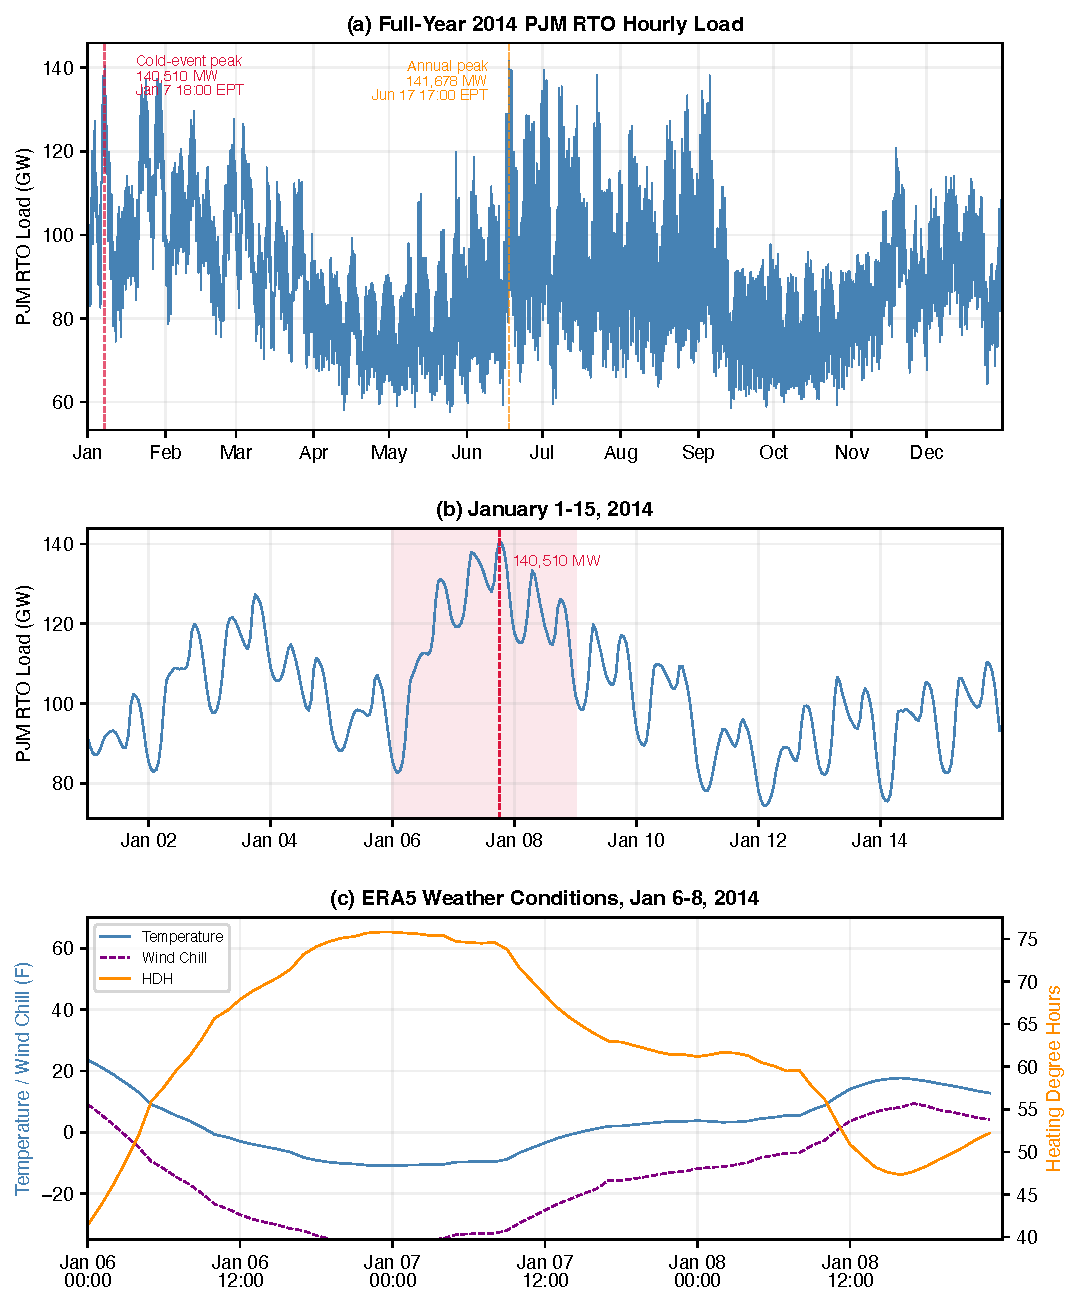
\includegraphics[width=\textwidth]{figures/figure1_event_definition}
\caption{PJM RTO hourly load and ERA5 weather conditions during the January 2014 Polar Vortex. Panel (a) shows full-year 2014 PJM RTO metered load, with the cold-event peak (140,510 MW, Jan 7 18:00 EPT) and the 2014 annual peak (141,678 MW, Jun 17 17:00 EPT) marked. Panel (b) shows the Jan 1--15 zoom with the Jan 6--8 event window shaded. Panel (c) shows ERA5 great\_lakes\_core temperature, wind chill, and heating degree hours (HDH) during the Jan 6--8 event window. All load data are from PJM Data Miner 2; weather data are same-hour ERA5 retrospective reanalysis.}
\label{fig:figure1}
\end{figure}

\clearpage
\section{Forecasting Framework}
\subsection{Forecasting Problem Formulation}
The forecasting task is defined as short-term hourly load forecasting: given calendar features, lagged load information, and same-hour ERA5 retrospective reanalysis weather inputs, produce estimates of PJM RTO metered load (actual\_load\_mw) for each hour in the evaluation period. The target variable is the hourly metered aggregate load across the full PJM transmission system, measured in megawatts.
For point forecast models, the prediction at hour $t$ is a single-valued estimate $\hat{y}_t$ of expected load. For probabilistic models, the prediction at hour $t$ is a set of conditional quantile estimates $\hat{q}_{\tau}(t)$, where $\tau \in (0,1)$ denotes the quantile level. A conditional quantile estimate $\hat{q}_{\tau}(t)$ targets the value below which a fraction $\tau$ of possible load outcomes would fall, conditional on the available features at hour $t$.
Quantile forecasts are evaluated using the pinball loss function. For a given quantile level $\tau$ and observed load $y_t$, the pinball loss is:
\[
\mathcal{L}_{\tau}(y_t,\hat{q}_{\tau}(t)) =
\begin{cases}
(1-\tau)\left(\hat{q}_{\tau}(t)-y_t\right), & y_t < \hat{q}_{\tau}(t), \\[4pt]
\tau\left(y_t-\hat{q}_{\tau}(t)\right), & y_t \geq \hat{q}_{\tau}(t).
\end{cases}
\]
The pinball loss penalizes over-estimation and under-estimation asymmetrically according to $\tau$: at high quantile levels, under-estimation is penalized more heavily than over-estimation. The mean pinball loss averaged across quantile levels summarizes overall probabilistic forecast skill. The Winkler score is used to evaluate prediction interval sharpness and coverage jointly and is reported alongside empirical coverage rates in Section 5.
Evaluation is reported for two windows: the full calendar year 2014 and the 72-hour January 6–8, 2014 polar vortex window defined in Section 2.4. 

All weather-informed model results use same-hour ERA5 retrospective reanalysis weather input and reflect an idealized retrospective weather-information setting rather than an operational forecast-weather setting.


\subsection{Feature Construction}
The three trained models in this study --- Linear Regression, GBoost, and QR-GBT --- share a common 14-feature input structure. Features are constructed from three sources: calendar information derived from the timestamp, lagged and rolling load values derived from the PJM hourly load series, and weather variables derived from the ERA5 great\_lakes\_core retrospective reanalysis fields described in Section 2.2. Naive baselines use only their defining lagged load values as described in Section 3.3 and do not use this feature set.
Calendar features capture the systematic diurnal, weekly, and seasonal structure of electricity demand:

\begin{itemize}[leftmargin=*, itemsep=2pt]
    \item \texttt{hour} --- hour of day (0--23), capturing the diurnal load cycle.
    \item \texttt{day\_of\_week} --- day of week (0--6), capturing weekday and weekend demand patterns.
    \item \texttt{month} --- calendar month (1--12), capturing seasonal load variation.
    \item \texttt{is\_weekend} --- binary indicator for Saturday and Sunday, capturing the structural load reduction on non-business days.
\end{itemize}


Lag and rolling load features capture demand persistence and load memory at multiple timescales:

\begin{itemize}[leftmargin=*, itemsep=2pt]
    \item \texttt{load\_lag\_1h} --- load observed one hour prior, capturing short-term persistence.
    \item \texttt{load\_lag\_24h} --- load observed 24 hours prior, capturing same-hour-previous-day patterns.
    \item \texttt{load\_lag\_168h} --- load observed 168 hours (one week) prior, capturing same-hour-previous-week patterns.
    \item \texttt{rolling\_mean\_24h} --- arithmetic mean of load over the preceding 24 hours, summarizing recent short-term baseline load.
    \item \texttt{rolling\_mean\_168h} --- arithmetic mean of load over the preceding 168 hours, summarizing the recent weekly baseline load level.
\end{itemize}


Weather features are derived from ERA5 t2m, u10, and v10 fields aggregated over the great\_lakes\_core grid box as described in Section 2.2. Dewpoint temperature (d2m) was not downloaded and is not used. NOAA ISD station data are not used in the modeling table:

\begin{itemize}[leftmargin=*, itemsep=2pt]
    \item \texttt{t\_f} --- 2-metre air temperature in degrees Fahrenheit, the primary thermal demand driver.
    \item \texttt{wc\_f} --- wind chill in degrees Fahrenheit, computed using the NOAA/NWS formula when $T \leq 50^\circ$F and wind speed exceeds 3 mph, otherwise equal to \texttt{t\_f}; captures the additional heating demand effect of cold wind.
    \item \texttt{ws} --- wind speed in mph, computed as $\sqrt{u_{10}^2 + v_{10}^2}$ converted from m/s; provides wind information relevant to wind chill and cold-stress feature construction.
    \item \texttt{hdh} --- heating degree hours, computed as $\max(65 - T^\circ\mathrm{F}, 0)$; a non-negative hourly measure of heating demand pressure.
    \item \texttt{cdh} --- cooling degree hours, computed as $\max(T^\circ\mathrm{F} - 65, 0)$; a non-negative hourly measure of cooling demand pressure.
\end{itemize}


Feature construction respects chronological ordering throughout. No future observations are used in constructing the feature value for the prediction target at hour $t$. No 2014 observations are used for model training. The complete feature set is summarized alongside model specifications in Table 2.
\subsection{Point Forecast Baselines}
Five point forecast models are evaluated, ranging from naive reference baselines to a trained machine learning model. PJM Day-Ahead load forecasts are included as an external operational benchmark.
\begin{description}[leftmargin=!, labelwidth=3.4cm, itemsep=4pt]
\item[Persistence-1h] Predicts hour $t$ load as equal to the load observed at hour $t - 1$. This model requires no training and uses no weather input; it serves as a lower-bound reference representing the simplest possible extrapolation from the most recent observation.
\item[Naive-24h] Predicts hour $t$ load as equal to the load observed at the same hour on the previous day (hour $t - 24$). This model requires no training and captures the diurnal cycle without any explicit weather or calendar modeling.
\item[Naive-168h] Predicts hour $t$ load as equal to the load observed at the same hour one week prior (hour $t - 168$). This model requires no training and captures both the diurnal cycle and the weekly schedule pattern; it is often a stronger naive baseline than Naive-24h during periods of stable weekly demand structure.
\item[Linear Regression] Is a multivariate linear model fitted to the full 14-feature set described in Section 3.2 using ordinary least squares on the 2010–2013 training data. It uses the same ERA5 retrospective weather inputs as the machine learning models and serves as a parametric reference point for assessing the marginal contribution of nonlinear tree-based modeling.
\item[GBoost] Is a gradient boosted regression tree model fitted on the same 14-feature training set. Gradient boosted trees construct an ensemble of shallow decision trees in a stagewise additive manner, with each successive tree fitted to the residuals of the preceding ensemble \cite{friedman2001greedy}. This approach captures nonlinear feature interactions --- including the nonlinear load-temperature relationship at temperature extremes --- without requiring explicit interaction terms or polynomial feature expansion. GBoost is trained on the 2010–2013 data and uses the same ERA5 retrospective reanalysis weather inputs as the linear model; all results reflect the retrospective setting.
\item[PJM Day-Ahead] Forecasts are obtained from PJM Data Miner 2 and represent the operational day-ahead load forecast issued by PJM using PJM's internal forecasting system and inputs not controlled by this study. PJM Day-Ahead forecasts are not produced by any model in this study and are included solely as an external benchmark to provide operational context for the point forecast results. PJM's internal inputs and methodology are not controlled by this study. No claim of operational superiority over PJM is made; the comparison is retrospective and the ERA5 retrospective setting gives the gradient boosted models an informational advantage not available in real-time operations.
\end{description}
\subsection{Quantile Regression Gradient-Boosted Trees}
Probabilistic forecasts are produced by a quantile regression gradient-boosted trees model (QR-GBT). Rather than minimizing squared error, QR-GBT fits a separate gradient boosted ensemble for each target quantile level by minimizing the pinball loss at that quantile \cite{koenker1978regression,friedman2001greedy}. This approach makes no parametric assumption about the conditional distribution of load and allows the width and asymmetry of prediction intervals to vary across hours, capturing the dependence of forecast uncertainty on weather conditions, time of day, and load level.
Seven quantile levels are estimated: q01, q05, q10, q50, q90, q95, and q99. The q50 estimate serves as the QR-GBT median forecast. Nominal prediction intervals are constructed from paired quantiles:


\begin{itemize}[leftmargin=*, itemsep=2pt]
    \item The nominal 90\% prediction interval is bounded by the q05 lower quantile and the q95 upper quantile.
    \item The nominal 98\% prediction interval is bounded by the q01 lower quantile and the q99 upper quantile.
\end{itemize}


All seven quantile models are trained on the 2010–2013 training data using the same 14-feature input structure described in Section 3.2 and the same ERA5 retrospective reanalysis weather inputs. Model specifications are summarized in Table 2.
\subsection{Prediction Interval Construction and Quantile Crossing Correction}
A known limitation of independently fitted quantile regression models is quantile crossing: individual quantile estimates fitted separately at different levels are not constrained to be monotonically ordered, and an estimated lower quantile may exceed an estimated upper quantile at some hours. Quantile crossing produces prediction intervals that violate the required monotonicity of a valid cumulative distribution function.
In the full-year 2014 test set, quantile crossing was detected in 5,786 of 8,760 test hours, representing 66\% of all evaluation hours. This crossing rate is substantial and indicates that the independently fitted quantile models produce inconsistent orderings across a large fraction of the test period.


Post-hoc monotonic rearrangement was applied to enforce non-decreasing quantile order across the seven estimated quantiles at each hour. All prediction interval coverage rates and Winkler scores reported in Section 5 are computed using the rearranged quantile estimates. 

This correction is post-hoc and should be treated as a methodological limitation: it restores a necessary ordering property but does not guarantee well-calibrated prediction intervals, particularly under distribution-shifting conditions such as an extreme cold-weather event. The implications of this high crossing rate for interval coverage during the polar vortex window are examined in the evaluation results.
\subsection{Workflow Summary}
Figure 2 presents a conceptual diagram of the end-to-end forecasting and evaluation workflow (figure2\_workflow.pdf). The pipeline proceeds from two public data sources --- PJM Data Miner 2 hourly load records and ERA5 retrospective reanalysis weather fields --- through feature construction as described in Sections 2 and 3.2, into parallel point forecast and quantile regression model fitting on the 2010–2013 training period, and finally into evaluation against the held-out 2014 test set across both the full-year and polar vortex event windows. Figure 2 is a conceptual schematic and contains no data-derived numerical results; all evaluation outputs are reported in Section 5.

\begin{table}[htbp]
\centering
\caption{Models evaluated. All weather-informed models use ERA5 retrospective reanalysis (not operational forecast). For quantile models, post-hoc monotonic rearrangement was applied to correct quantile crossings (66\% of test hours affected).}
\label{tab:model_summary}
\begin{tabular}{lllll}
\toprule
Model & Type & Weather Input & Training & Role \\
\midrule
Persistence-1h & Naive baseline & None & None & Lower bound \\
Naive-24h & Seasonal naive & None & None & Seasonal benchmark \\
Naive-168h & Weekly naive & None & None & Weekly benchmark \\
GBoost & Point forecast & ERA5 reanalysis & 2010--2013 & Point benchmark \\
QR-GBT & Quantile (q01--q99) & ERA5 reanalysis & 2010--2013 & Prob. forecast \\
PJM Day-Ahead & Operational & PJM internal & N/A & External benchmark \\
\bottomrule
\end{tabular}
\end{table}

% Figure 2
\begin{figure}[htbp]
\centering
\includegraphics[width=\textwidth]{figures/figure2\_workflow}
\caption{Conceptual workflow diagram illustrating the forecasting and evaluation pipeline. Official PJM RTO load (2010--2014) and ERA5 retrospective reanalysis weather are combined via feature engineering (calendar variables, load lags, rolling means, and weather features) and passed to point baseline models and QR-GBT quantile models. Evaluation compares full-year 2014 performance against Jan 6--8 Polar Vortex stress-window performance and against the PJM day-ahead forecast as an external benchmark. Figure 2 is a conceptual schematic and contains no data-derived numerical results.}
\label{fig:figure2}
\end{figure}

\section{Experimental Design and Evaluation Protocol}
\subsection{Training and Test Partition}
The experimental design follows a strict chronological holdout structure. The full dataset spans January 1, 2010 through December 31, 2014, yielding 43,824 hourly observations prior to feature construction. Following the creation of lagged and rolling-window features with a maximum lookback of 168 hours, the first 168 observations are dropped to avoid partially undefined feature rows, leaving 43,656 complete observations.
The training period covers January 1, 2010 through December 31, 2013 (34,896 observations). The test period covers the full calendar year 2014 (8,760 observations). No 2014 observations are used for model fitting. Any hyperparameter selection procedure must be documented separately and must not use held-out 2014 outcomes. The training leakage count is zero.
Within the test period, earlier observed load values are used as lagged inputs for later test hours where chronologically valid --- for example, the load observed at hour $t - 24$ is a legitimate input when predicting hour $t$. This is a standard property of autoregressive feature structures and does not constitute training leakage, as no model parameters are updated using test-period data.
All three trained models --- Linear Regression, GBoost, and QR-GBT --- are fitted exclusively on training-period observations. The three naive baselines (Persistence-1h, Naive-24h, Naive-168h) require no fitting procedure. The PJM Day-Ahead forecast is obtained as an external benchmark and is not produced or fitted by this study.
\subsection{Evaluation Windows}
Forecast performance is evaluated across three defined windows, each serving a distinct purpose in the evaluation design.

\begin{description}[leftmargin=!, labelwidth=4.8cm, itemsep=4pt]
\item[Full-year 2014 test set] The primary evaluation window is the complete 8,760-hour 2014 test year. Full-year metrics provide an aggregate characterization of model performance across the full range of operating conditions present in 2014, including moderate-load periods, shoulder seasons, summer peaks, and the January cold event. Full-year metrics are reported for all models.

\item[January 6--8, 2014 vortex window] The stress-test evaluation window is the 72-hour period from 00:00 EPT January 6, 2014 through 23:00 EPT January 8, 2014. The January 6–8, 2014 Polar Vortex produced a near-annual-peak RTO load of 140,510.2 MW at Jan 7 18:00 EPT, equal to 99.18\% of the 2014 annual peak of 141,677.9 MW recorded on Jun 17 17:00 EPT. This window is defined as a near-annual-peak cold-weather stress event and evaluated separately to assess whether full-year aggregate metrics adequately characterize model behavior under extreme cold conditions. Event-window metrics are reported for all models.
\item[June 16--18, 2014 summer window] The comparison window is the 72-hour period from 00:00 EPT June 16, 2014 through 23:00 EPT June 18, 2014, which contains the 2014 annual peak of 141,677.9 MW. This window is evaluated in parallel with the cold-event window to distinguish between general peak-load forecasting difficulty and the specific challenge of extreme cold-weather generalization. Comparing results across the two near-peak windows --- one cold-driven, one heat-driven --- allows the evaluation to assess whether any performance degradation observed during the polar vortex window is attributable to peak-load conditions generally or to the out-of-distribution character of the cold event specifically.
\item[Top 1\% load hours] As a supplementary high-load subset, the top 1\% of 2014 test hours by observed load level (approximately 88 hours) may be used in Section 5 to characterize forecast calibration across the upper tail of the 2014 load distribution. This subset is not a primary evaluation window.
\end{description}

All weather-informed model results across all evaluation windows use same-hour ERA5 retrospective reanalysis weather input. This is an idealized retrospective weather-information setting and is not an operational forecast-weather setting. The evaluation does not quantify degradation from weather forecast error, and results should not be interpreted as achievable under real-time operational conditions.
\subsection{Point Forecast Evaluation Metrics}
Point forecast accuracy is evaluated using two primary metrics: mean absolute error (MAE) and root mean squared error (RMSE). Both metrics are computed over all hours within each evaluation window.

\begin{description}[leftmargin=!, labelwidth=3.2cm, itemsep=4pt]
\item[MAE] The average of the absolute differences between observed and predicted load across all hours in the evaluation window, expressed in megawatts. MAE is the primary point forecast accuracy metric throughout this study.
\item[RMSE] The square root of the average squared differences between observed and predicted load. RMSE applies greater weight to large errors than MAE. Because the polar vortex event produces concentrated large errors at peak hours, RMSE provides additional sensitivity to these tail errors relative to MAE.
\item[Error convention] Forecast error at hour $t$ is defined as actual minus predicted: $e_t = y_t - \hat{y}_t$. A positive error indicates underprediction; a negative error indicates overprediction. This convention is applied consistently across all error reporting and directional analysis.
\item[Event-peak error] For the polar vortex evaluation window, the point forecast error at the peak hour (Jan 7 18:00 EPT, observed load 140,510.2 MW) is reported individually for each model in Table 5. This single-hour error is distinct from the window-level MAE and RMSE and is reported alongside the probabilistic interval inclusion check described in Section 4.4.
Point forecast results for all models and all evaluation windows are reported in Table 3.
\end{description}
\subsection{Probabilistic Forecast Evaluation Metrics}
Probabilistic forecast evaluation is applied to the QR-GBT model. All probabilistic evaluation uses the post-hoc rearranged quantile estimates, as described in Section 3.5. As noted there, quantile crossing was detected in 5,786 of 8,760 full-year 2014 test hours (66\% of test hours) prior to rearrangement. The rearrangement correction is a methodological limitation and does not guarantee well-calibrated intervals.
The following metrics are defined and reported in Section 5.

\begin{description}[leftmargin=!, labelwidth=3.5cm, itemsep=4pt]
\item[q50 MAE] The MAE of the QR-GBT q50 (median) forecast, computed using the same definition as the point forecast MAE in Section 4.3. This allows direct comparison of the QR-GBT median forecast with the GBoost and Linear Regression point forecasts on a common accuracy scale.
\item[Mean pinball loss] Mean pinball loss is computed by averaging the pinball loss --- defined in Section 3.1 --- over all evaluated hours and over the seven estimated quantile levels: q01, q05, q10, q50, q90, q95, and q99. Lower mean pinball loss indicates better overall probabilistic forecast skill across the full quantile set. Mean pinball loss is reported by evaluation window.
\item[Empirical coverage] Empirical coverage is the fraction of evaluation hours for which the observed load falls within the estimated interval bounds. For the nominal 90\% prediction interval, the bounds are the q05 lower quantile and the q95 upper quantile. For the nominal 98\% prediction interval, the bounds are the q01 lower quantile and the q99 upper quantile. A well-calibrated model should achieve empirical coverage close to its nominal level. Systematic undercoverage --- empirical coverage materially below the nominal level --- indicates that the estimated intervals are too narrow relative to the actual conditional uncertainty. Empirical coverage rates are reported by evaluation window in Section 5.
\item[Winkler score] The Winkler score evaluates prediction interval sharpness and interval violations jointly. It rewards narrower intervals when observations fall inside the interval bounds, and penalizes observations that fall outside the interval in proportion to the exceedance distance. The penalty magnitude scales with the nominal miscoverage rate, so that violations of higher-confidence intervals are penalized more heavily. Lower mean Winkler score indicates better joint sharpness and coverage. The Winkler score is reported for the nominal 90\% prediction interval across all evaluation windows.
\item[Event-peak interval check] For the polar vortex peak hour (Jan 7 18:00 EPT, observed load 140,510.2 MW), the evaluation records whether the observed load falls within each estimated prediction interval. This is a binary inclusion check, reported in Table 5 for both the nominal 90\% interval (q05–q95 bounds) and the nominal 98\% interval (q01–q99 bounds). The post-rearrangement q95 and q99 estimates at the peak hour are also reported in Table 5 to allow direct comparison with the observed peak load.
Full probabilistic evaluation results for all windows are reported in Table 4. Event-peak probabilistic results are reported in Table 5.
\end{description}
\subsection{Benchmark Comparisons and Interpretation Rules}
The evaluation compares multiple models across point forecast and probabilistic forecast tasks. Several interpretation rules govern how these comparisons should be read.

\begin{description}[leftmargin=!, labelwidth=3.6cm, itemsep=4pt]
\item[Naive baselines] The three naive baselines --- Persistence-1h, Naive-24h, and Naive-168h --- require no training and use only their defining lagged load values. These baselines provide reference points for assessing whether trained models add value beyond simple load-memory rules. These comparisons are evaluated using MAE across all windows.
\item[PJM Day-Ahead] The PJM Day-Ahead forecast is an external benchmark produced operationally by PJM using PJM's internal forecasting system and inputs not controlled by this study. It is included to provide operational context for the point forecast results. GBoost and QR-GBT use same-hour ERA5 retrospective reanalysis weather input, which gives these models an informational advantage not available under real-time operational conditions. Accordingly, comparisons with PJM Day-Ahead are retrospective and should not be interpreted as evidence of operational superiority. The purpose of the comparison is to contextualize the magnitude of retrospective gradient boosted model errors relative to those of an operational forecasting system during the same event.
\item[Full-year vs. event-window] The comparison between full-year and event-window metrics is used to assess whether aggregate annual evaluation masks stress-window behavior. Section 5 reports both sets of metrics for all applicable models, and the two should be read in conjunction rather than treated as independent summaries.
\item[Retrospective weather] All comparisons involving GBoost or QR-GBT are subject to the constraint that these models use same-hour ERA5 retrospective reanalysis weather input. This is not an operational forecast-weather setting. No comparison in this study quantifies the additional error that would arise from replacing retrospective reanalysis weather with real-time NWP forecast weather.
\end{description}

\subsection{Reproducibility and Leakage Controls}
All primary data inputs used in this study are publicly available. PJM RTO hourly metered load data are available from PJM Data Miner 2. ERA5 reanalysis fields are available from the Copernicus Climate Data Store \cite{hersbach2020era5}. The ERA5 great\_lakes\_core spatial aggregation procedure is defined in src/data/process\_era5\_2014.py as described in Section 2.2.
The following leakage controls are applied throughout the experimental design:

\begin{itemize}[leftmargin=*, itemsep=2pt]
    \item No 2014 observations are used for model fitting.
    \item Lag and rolling features are constructed using only observations at hours strictly prior to the prediction target hour $t$, respecting chronological ordering at all times.
    \item The 168-hour trim at the start of the dataset ensures that no partially defined feature rows are included in training or evaluation.
    \item The training and test periods are defined by calendar year boundaries and are non-overlapping.
\end{itemize}


These controls ensure that point and probabilistic forecast errors in Section 5 reflect genuine out-of-sample generalization from models fitted on 2010–2013 data and evaluated against held-out 2014 conditions, including the January 6–8 polar vortex event defined in Section 2.4.

\section{Results}
\subsection{Point Forecast Accuracy}
Table 3 reports MAE and RMSE for all five point forecast models and the PJM Day-Ahead external benchmark across the full-year 2014 test set and the January 6–8 vortex window. 

All weather-informed model results use same-hour ERA5 retrospective reanalysis weather input and reflect an idealized retrospective weather-information setting rather than an operational forecast-weather setting.


Across the full-year 2014 test set, GBoost achieves the lowest MAE (721 MW) and lowest RMSE (994 MW) among all evaluated point forecasts. Linear Regression reduces full-year MAE to 2,354 MW relative to Persistence-1h (2,745 MW), indicating that the weather and calendar features carry predictive value beyond one-hour load persistence. Naive-24h and Naive-168h produce substantially higher full-year errors (5,960 MW and 8,009 MW MAE respectively), confirming that models using only load-memory rules without weather or calendar inputs are inadequate as standalone forecasts over a full annual cycle.
PJM Day-Ahead produces a full-year MAE of 1,937 MW. GBoost produces a full-year MAE of 721 MW. This difference reflects the retrospective informational advantage conferred by same-hour ERA5 reanalysis weather inputs; it does not constitute evidence of operational superiority, as PJM Day-Ahead is produced in real time using forecast-weather inputs not controlled by this study.
During the January 6–8 vortex window, GBoost again produces the lowest MAE (1,705 MW) and RMSE (2,037 MW) among evaluated point forecasts. However, all models show error degradation relative to their full-year performance, indicating that the cold-event window presents greater forecasting difficulty across the board. The degradation is most severe for the seasonal naive baselines: Naive-24h MAE increases from 5,960 MW full-year to 15,598 MW during the vortex window, and Naive-168h MAE increases from 8,009 MW to 24,531 MW. Linear Regression vortex MAE (4,248 MW) is approximately 1.8 times its full-year MAE (2,354 MW). GBoost vortex MAE (1,705 MW) is approximately 2.4 times its full-year MAE (721 MW). PJM Day-Ahead vortex MAE (3,148 MW) is approximately 1.6 times its full-year MAE (1,937 MW). The relative degradation pattern across models is discussed further in Section 6.


\subsection{Event-Peak Point Forecast Errors}
The January 6–8, 2014 Polar Vortex produced a near-annual-peak RTO load of 140,510.2 MW at Jan 7 18:00 EPT, equal to 99.18\% of the 2014 annual peak of 141,677.9 MW recorded on Jun 17 17:00 EPT. Table 5 reports the point forecast and prediction interval results at this single peak hour.
Using the error convention $e_t = y_t - \hat{y}_t$ (positive = underprediction, negative = overprediction), the point forecast errors at Jan 7 18:00 EPT are:


\begin{itemize}[leftmargin=*, itemsep=2pt]
    \item Persistence-1h: predicted 137,604~MW, error $+$2,906~MW (underprediction).


    \item Naive-24h: predicted 130,537~MW, error $+$9,973~MW (underprediction).


    \item Naive-168h: predicted 109,742~MW, error $+$30,769~MW (underprediction).


    \item Linear Regression: predicted 134,985~MW, error $+$5,525~MW (underprediction).


    \item GBoost: predicted 141,898~MW, error $-$1,388~MW (overprediction).


    \item PJM Day-Ahead: predicted 137,965~MW, error $+$2,545~MW (underprediction).
\end{itemize}


All models except GBoost underpredict the event peak. The seasonal naive baselines produce large positive errors consistent with their full-year vortex-window degradation: Naive-168h, anchored to load from the prior week rather than to the contemporaneous cold-event conditions, misses the event peak by 30,769 MW. Linear Regression underpredicts by 5,525 MW despite using the same ERA5 retrospective weather inputs as GBoost, suggesting that the linear specification was less able than GBoost to represent event-window behavior under extreme cold conditions. GBoost slightly overpredicts the event peak by 1,388 MW. PJM Day-Ahead underpredicts by 2,545 MW.
These single-hour results are not sufficient to characterize overall model behavior and should be read alongside the window-level MAE and RMSE in Table 3.
\subsection{Probabilistic Forecast Performance}
Table 4 reports QR-GBT probabilistic forecast metrics across the full-year 2014 test set, the January 6–8 vortex window, the June 16–18 summer near-peak window, and the top 1\% load-hour subset. All probabilistic evaluation uses post-hoc rearranged quantile estimates as described in Section 3.5; reported prediction intervals should be interpreted in light of the high quantile crossing rate (5,786 of 8,760 full-year test hours, 66\%) prior to rearrangement.


Full-year 2014. The QR-GBT q50 median forecast achieves a full-year MAE of 761 MW, close to the GBoost point forecast MAE of 721 MW. The nominal 90\% prediction interval (q05–q95) achieves an empirical coverage rate of 86.8\% against a nominal target of 90\%. The nominal 98\% prediction interval (q01–q99) achieves an empirical coverage rate of 97.3\%. The mean pinball loss averaged across the seven estimated quantile levels is 153, and the mean Winkler score for the nominal 90\% interval is 4,627 MW.
January 6–8 vortex window. During the vortex window, the q50 MAE increases to 2,130 MW. The nominal 90\% PI empirical coverage falls to 66.7\%, 20.1 percentage points below its full-year rate and 23.3 percentage points below the nominal 90\% target. The nominal 98\% PI empirical coverage falls to 84.7\%, 12.6 percentage points below its full-year rate and 13.3 percentage points below the nominal 98\% target. The mean pinball loss increases to 473 and the mean Winkler score for the nominal 90\% interval increases to 15,476 MW, indicating poorer joint interval sharpness and coverage performance relative to the full-year evaluation.
June 16–18 summer near-peak window. The q50 MAE during the summer near-peak window is 1,060 MW. The nominal 90\% PI coverage is 86.1\% and the nominal 98\% PI coverage is 93.1\%. The mean pinball loss is 209 and the Winkler score for the nominal 90\% interval is 6,355 MW.


Top 1\% load hours. The top 1\% of 2014 test hours by observed load (approximately 88 hours) show 90\% PI coverage of 63.2\% and 98\% PI coverage of 82.8\%. The q50 MAE for this subset is 2,539 MW, the mean pinball loss is 502, and the Winkler score for the nominal 90\% interval is 16,168 MW. These results are consistent with the vortex-window findings and indicate that coverage degradation is not limited to the polar vortex event; it also appears in the top 1\% load-hour subset of the 2014 evaluation year.
Figure 3 shows the QR-GBT retrospective probabilistic forecast during the January 6–8 vortex window, including the nominal 90\% and 98\% prediction interval bands and the observed load series. As shown in Figure 3, the event peak at Jan 7 18:00 EPT falls outside the nominal 98\% prediction interval. All forecast values in Figure 3 use same-hour ERA5 retrospective reanalysis weather input.
\subsection{Calibration Breakdown Across Evaluation Windows}
Figure 4 summarizes empirical coverage rates across evaluation windows for the nominal 90\% and 98\% prediction intervals. The full-year 90\% PI coverage rate of 86.8\% is reasonably close to the nominal 90\% target, which might suggest adequate probabilistic calibration under a single-number summary. However, disaggregation by evaluation window reveals that this aggregate rate masks substantial undercoverage during periods of high and extreme load.
The nominal 90\% PI coverage falls from 86.8\% (full-year) to 66.7\% during the vortex window --- a decline of 20.1 percentage points. The nominal 98\% PI coverage falls from 97.3\% (full-year) to 84.7\% during the vortex window. The top 1\% load-hour subset shows 90\% PI coverage of 63.2\% and 98\% PI coverage of 82.8\%, similar in magnitude to the vortex window findings. The summer near-peak window 90\% PI coverage (86.1\%) is close to the full-year rate and does not show the same pattern of degradation.


These results indicate that aggregate full-year calibration metrics do not adequately characterize probabilistic forecast performance during the high-load and extreme cold-weather conditions that are operationally most consequential. The mechanisms underlying this calibration breakdown are examined in Section 6.
\subsection{Winter versus Summer Near-Peak Comparison}
Figure 5 places the January 6–8 vortex window results alongside the June 16–18 summer near-peak window results. The two windows have similar peak-load magnitudes: the winter vortex peak is 140,510 MW and the summer peak is 141,678 MW, a difference of 1,168 MW or less than 1\% of the summer peak. Despite this similarity in peak magnitude, probabilistic performance is materially worse during the cold-event window than during the summer near-peak window across all reported metrics.
The q50 MAE during the vortex window (2,130 MW) is approximately twice the q50 MAE during the summer window (1,060 MW). The mean pinball loss during the vortex window (473) is approximately twice that of the summer window (209). The nominal 90\% PI Winkler score during the vortex window (15,476 MW) is approximately 2.4 times that of the summer window (6,355 MW). Nominal 90\% PI coverage is 66.7\% during the vortex window and 86.1\% during the summer window; nominal 98\% PI coverage is 84.7\% and 93.1\% respectively.
The comparison indicates that peak-load magnitude alone does not account for the degradation in probabilistic performance during the vortex window. The additional difficulty associated with the cold-event window, relative to a summer near-peak window of comparable load magnitude, is addressed in the Discussion.
\subsection{Tail-Risk Event-Peak Interval Check}
Table 5 and Figure 6 report the QR-GBT prediction interval bounds at the event peak hour (Jan 7 18:00 EPT, observed load 140,510 MW). All reported values use post-hoc rearranged quantile estimates as described in Section 3.5.
At the event peak, the QR-GBT q50 estimate is 135,357 MW, reflecting a median forecast underprediction of 5,153 MW. The post-rearrangement q95 estimate is 139,410 MW and the post-rearrangement q99 estimate is 139,585 MW. At the event peak, the observed load exceeded the post-rearrangement QR-GBT q99 estimate of 139,585 MW, leaving the event peak outside the nominal 98\% prediction interval. The q99 estimate falls 925 MW below the observed peak load of 140,510 MW.
The event peak also falls above the post-rearrangement q95 bound of 139,410 MW, confirming that the observed load at this hour lies outside the nominal 90\% prediction interval as well. Figure 6 illustrates the relationship between the observed event peak and the estimated quantile bounds at this hour.
These results indicate that at the hour of maximum cold-event load, the QR-GBT upper quantile estimates were insufficient to bound the observed outcome even at the 99th percentile level. The interpretation of this finding in terms of training-distribution coverage and the retrospective weather-input setting is addressed in Section 6.

\begin{table}[htbp]
\centering
\caption{Point forecast performance. All values in MW. Jan~7 18:00 EPT is the official cold-event peak (140,510~MW). The GBoost and Linear models use ERA5 retrospective reanalysis weather features.}
\label{tab:point_metrics}
\begin{tabular}{lrrrrr}
\toprule
Model & FY MAE & FY RMSE & Vort. MAE & Vort. RMSE & Peak Error \\
\midrule
Persistence-1h & 2,745 & 3,542 & 2,805 & 3,565 & $+$2,906 \\
Naive-24h & 5,960 & 8,105 & 15,598 & 18,645 & $+$9,973 \\
Naive-168h & 8,009 & 10,871 & 24,531 & 26,409 & $+$30,769 \\
Linear & 2,354 & 3,027 & 4,248 & 5,100 & $+$5,525 \\
GBoost & 721 & 994 & 1,705 & 2,037 & $-$1,388 \\
PJM Day-Ahead & 1,937 & 2,563 & 3,148 & 3,809 & $+$2,545 \\
\bottomrule
\end{tabular}
\end{table}

\begin{table}[htbp]
\centering
\caption{Probabilistic forecast performance of QR-GBT (q50 point, plus 90\% and 98\% prediction intervals). The 90\% PI coverage degrades from 86.8\% full-year to 66.7\% during the Polar Vortex. The official event peak (140,510~MW at Jan~7 18:00) falls outside the 98\% PI.}
\label{tab:prob_metrics}
\begin{tabular}{lrrrrr}
\toprule
Window & q50 MAE & Mean Pinball & 90\% PI Cov. & 98\% PI Cov. & Winkler (90\%) \\
\midrule
Full-year 2014 & 761 & 153 & 86.8\% & 97.3\% & 4,627 \\
Jan 6--8 Vortex & 2,130 & 473 & 66.7\% & 84.7\% & 15,476 \\
Jun 16--18 Summer & 1,060 & 209 & 86.1\% & 93.1\% & 6,355 \\
Top 1\% load hours & 2,539 & 502 & 63.2\% & 82.8\% & 16,168 \\
\bottomrule
\end{tabular}
\end{table}

\begin{table}[htbp]
\centering
\footnotesize
\caption{Prediction check at the official cold-event peak (Jan~7, 2014 18:00 EPT, 140,510~MW). Positive error means underprediction. The actual load exceeds the QR-GBT 98\% prediction interval.}
\label{tab:event_peak}
\begin{tabular}{lrrcc}
\toprule
Model & Pred. & Error & 90\% PI? & 98\% PI? \\
\midrule
PJM Day-Ahead & 137,965 & $+$2,545 & — & — \\
Persistence-1h & 137,604 & $+$2,906 & — & — \\
Naive-24h & 130,537 & $+$9,973 & — & — \\
GBoost point & 141,898 & $-$1,388 & — & — \\
QR-GBT q50 & 135,357 & $+$5,153 & Yes & No \\
QR-GBT q95 & 139,410 & $+$1,100 & No & No \\
QR-GBT q99 & 139,585 & $+$925 & No & No \\
\bottomrule
\end{tabular}
\end{table}

% Figure 3
\begin{figure}[htbp]
\centering
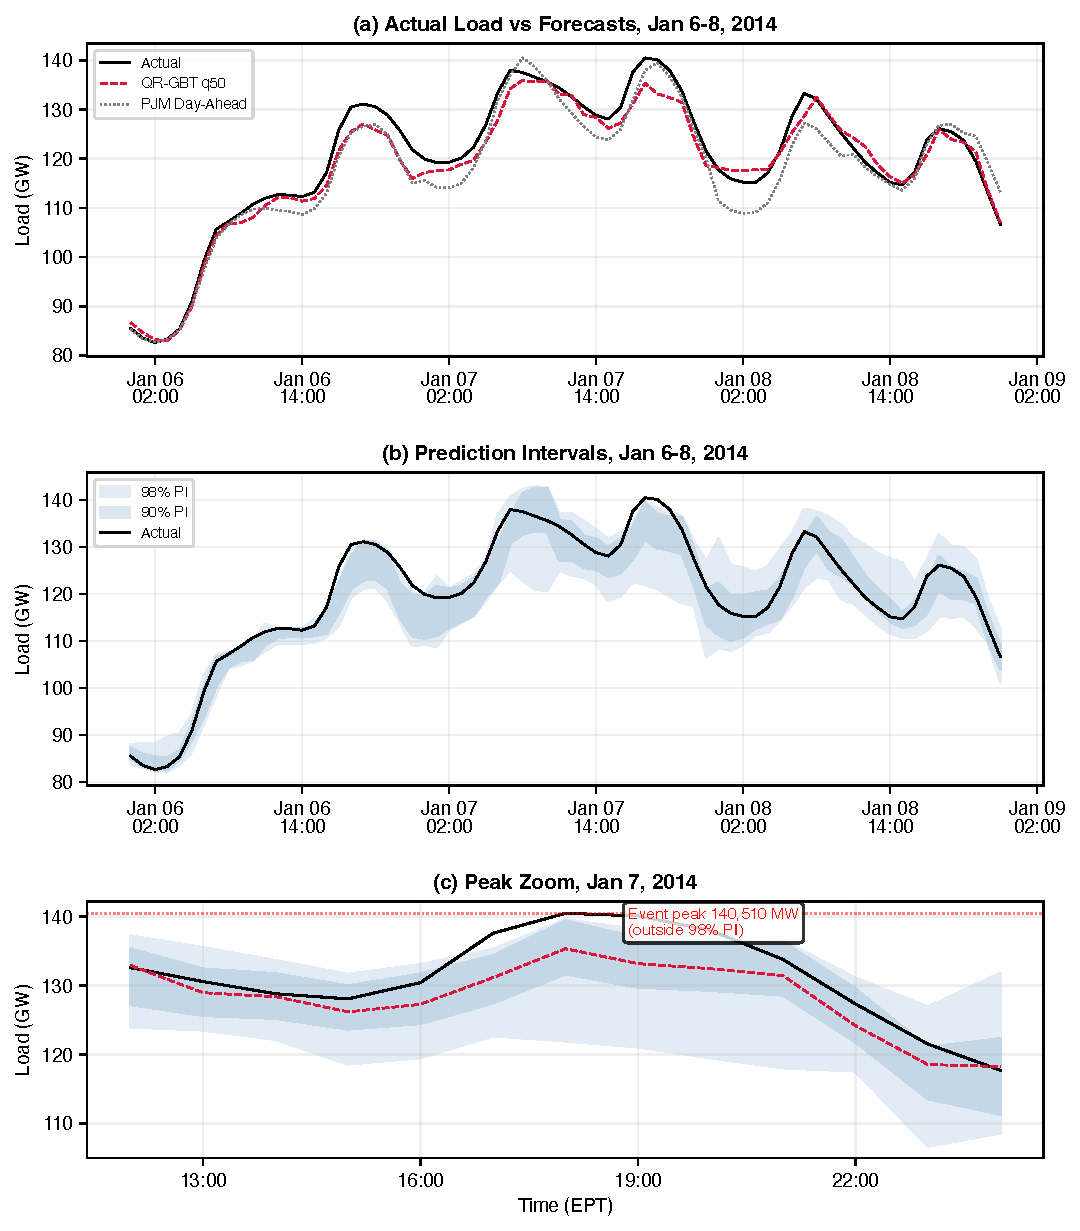
\includegraphics[width=\textwidth]{figures/figure3_vortex_quantile_forecast}
\caption{QR-GBT retrospective probabilistic forecast for the Jan 6--8, 2014 Polar Vortex event window (72 hours). Panel (a) compares actual PJM RTO load with the QR-GBT median (q50) forecast and the PJM day-ahead forecast. Panel (b) shows the 90\% and 98\% prediction intervals as shaded fans around the q50 forecast. Panel (c) zooms to Jan 7 18:00 EPT, the cold-event peak (140,510 MW); the actual load lies outside the nominal 98\% prediction interval. All model results use same-hour ERA5 retrospective reanalysis weather input. Prediction interval fill is approximate due to post-hoc monotonic quantile rearrangement applied to 66\% of test hours.}
\label{fig:figure3}
\end{figure}

% Figure 4
\begin{figure}[htbp]
\centering
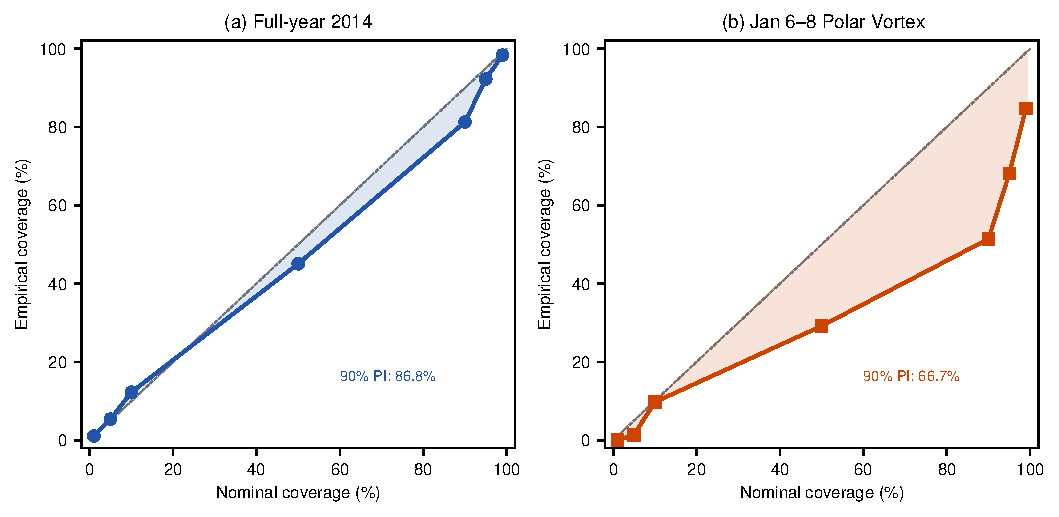
\includegraphics[width=\textwidth]{figures/figure4_calibration_breakdown}
\caption{Empirical coverage versus nominal quantile level for QR-GBT probabilistic forecasts. Panel (a) shows full-year 2014 calibration, where empirical coverage tracks the nominal diagonal reasonably well (90\% PI coverage = 86.8\%). Panel (b) shows the same calibration curve for the Jan 6--8 Polar Vortex window only, where empirical coverage falls substantially below nominal (90\% PI coverage = 66.7\%). All model results use same-hour ERA5 retrospective reanalysis weather input.}
\label{fig:figure4}
\end{figure}

% Figure 5
\begin{figure}[htbp]
\centering
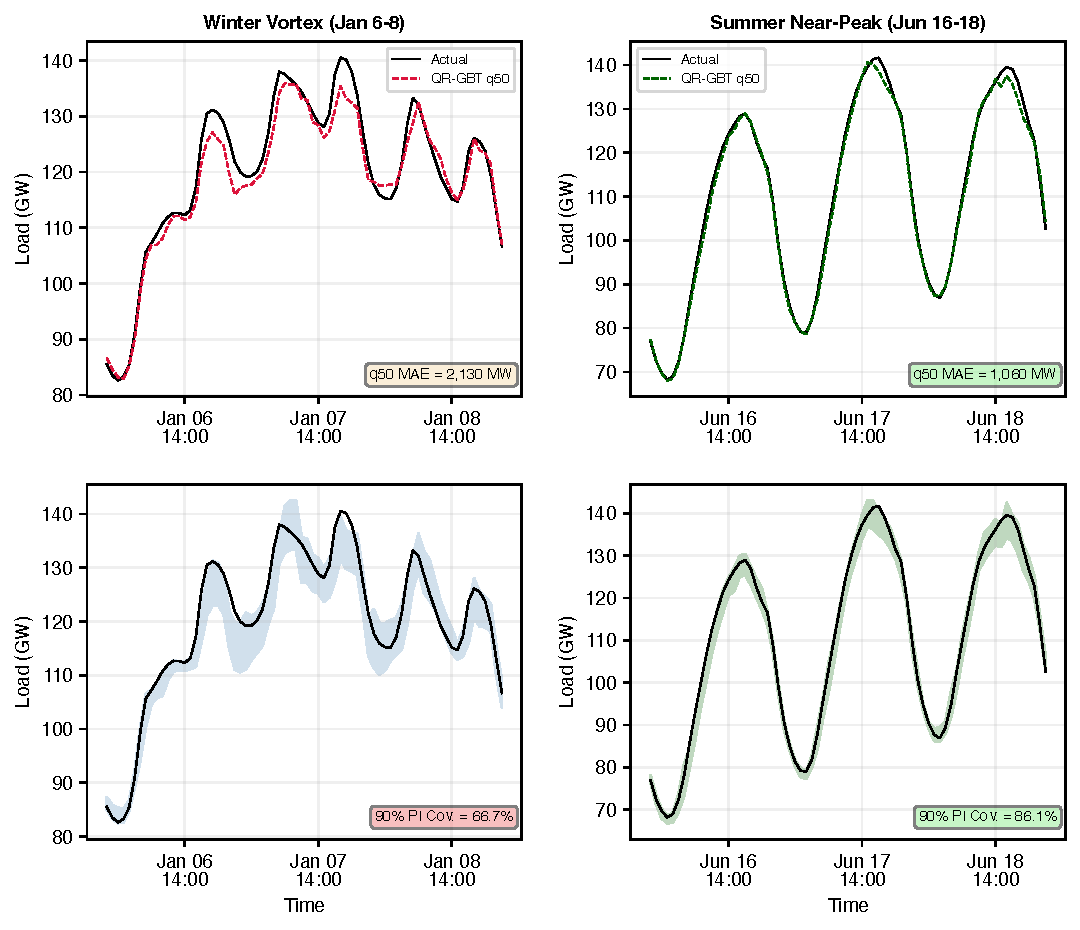
\includegraphics[width=\textwidth]{figures/figure5_winter_vs_summer}
\caption{Comparison of QR-GBT forecast performance between the Jan 6--8, 2014 cold-event window (winter vortex, peak 140,510 MW) and the Jun 16--18, 2014 near-peak window (summer, peak 141,678 MW). Despite similar load magnitudes, the vortex window exhibits substantially higher forecast difficulty: QR-GBT q50 MAE = 2,130 MW (vortex) versus 1,060 MW (summer), and 90\% PI coverage = 66.7\% (vortex) versus 86.1\% (summer). All model results use same-hour ERA5 retrospective reanalysis weather input. Prediction interval fill is approximate due to quantile crossing correction.}
\label{fig:figure5}
\end{figure}

% Figure 6
\begin{figure}[htbp]
\centering
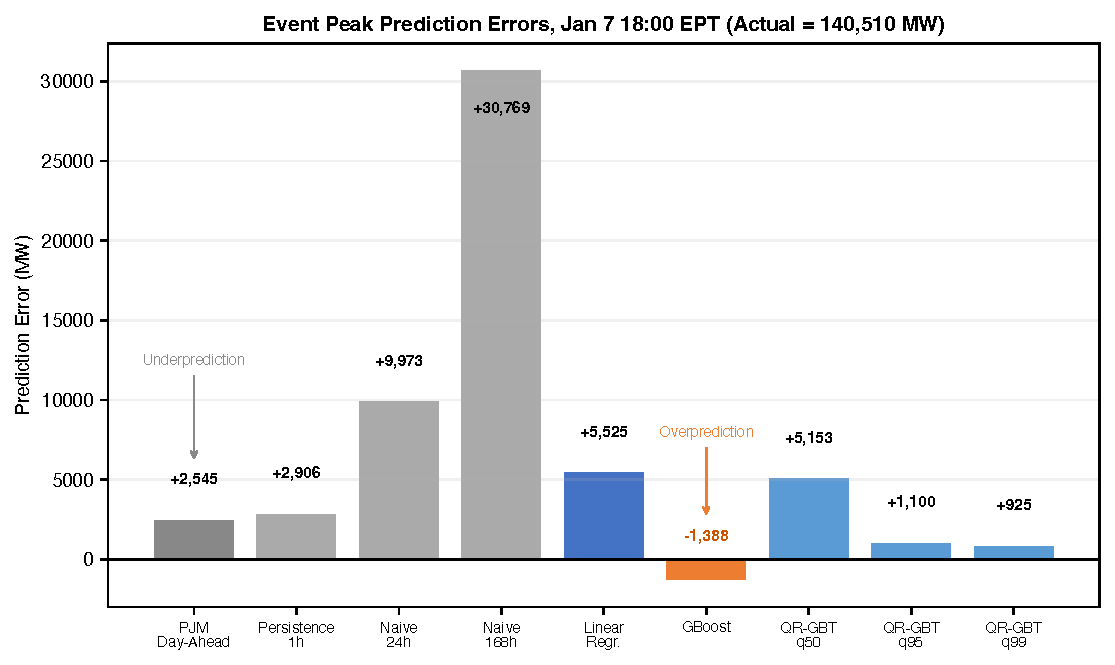
\includegraphics[width=\textwidth]{figures/figure6_tail_risk_event_peak}
\caption{Prediction errors at the official cold-event peak hour (Jan 7, 2014 18:00 EPT, actual load = 140,510 MW) for all evaluated models. Positive values indicate underprediction. The actual load exceeds the QR-GBT q99 upper quantile bound (139,585 MW) by 925 MW, falling outside the 98\% prediction interval. The QR-GBT q50 median forecast is 135,357 MW. All weather-informed model results use same-hour ERA5 retrospective reanalysis weather input.}
\label{fig:figure6}
\end{figure}

\clearpage
\section{Discussion}
\subsection{Full-Year Calibration Masks Event-Window Undercoverage}
The full-year 2014 QR-GBT results present a broadly acceptable calibration picture: the nominal 90\% prediction interval achieves an empirical coverage rate of 86.8\%, and the nominal 98\% prediction interval achieves 97.3\%. Evaluated solely on annual aggregate metrics, the probabilistic forecasts appear reasonably well-calibrated. Disaggregation by evaluation window, however, reveals that this aggregate summary conceals substantial undercoverage during the most operationally consequential period in the evaluation year.
During the January 6–8 vortex window, the nominal 90\% PI empirical coverage falls to 66.7\% --- a decline of 20.1 percentage points from the full-year rate and 23.3 percentage points below the nominal 90\% target. The nominal 98\% PI coverage falls to 84.7\%, more than 12 percentage points below its full-year rate. The top 1\% of load hours by observed load level shows consistent undercoverage: 90\% PI coverage of 63.2\% and 98\% PI coverage of 82.8\%. Coverage deteriorates during the conditions where accurate uncertainty quantification would be most consequential.


This pattern is consistent with a general risk in aggregate calibration assessment: when a high-frequency, moderate-load regime dominates the annual sample, aggregate coverage rates can appear adequate while masking systematic failures in lower-frequency, high-load regimes. In this case study, the full-year 2014 sample contains 8,760 hours; the vortex window represents only 72 of those hours, and the top 1\% subset approximately 88. The contribution of these hours to the aggregate coverage statistic is small, yet they represent the tail-risk conditions that probabilistic forecasts are most expected to address. These findings suggest that evaluation designs relying solely on full-year aggregate metrics may not surface stress-window calibration failures, and that window-specific coverage reporting provides material additional information.
\subsection{Extreme Cold as a Distribution-Shift Stress Test}
The January 6–8 polar vortex event constitutes a near-annual-peak cold-weather stress event within the 2014 evaluation year. The associated load conditions --- high sustained demand driven by intense cold, combined with near-peak load magnitudes --- are consistent with distribution-shift stress relative to more moderate operating conditions that make up the more moderate operating conditions that are expected to dominate many multi-year hourly samples. Whether the 2010–2013 training period contains weather events of comparable intensity is not directly verified here; this is addressed as a formal limitation in Section 7. The observed degradation in model performance during this window is consistent with the cold-event regime being underrepresented relative to more moderate operating conditions in the training data, but direct training-distribution support for this interpretation is not verified by this study.


All weather-informed model results use same-hour ERA5 retrospective reanalysis weather input. The performance degradation is observable across point and probabilistic forecast approaches: GBoost point forecast MAE increases from 721 MW full-year to 1,705 MW during the vortex window, approximately 2.4 times the full-year rate. QR-GBT q50 MAE increases from 761 MW to 2,130 MW. Mean pinball loss increases from 153 to 473.
The relative degradation of Naive-24h and Naive-168h is more severe, with vortex-window MAE reaching 15,598 MW and 24,531 MW respectively. These baselines anchor to load observed under different thermal conditions one day and one week prior, making them structurally ill-suited to events in which the driving weather conditions depart sharply from the recent past. Linear Regression, despite using the same retrospective ERA5 weather inputs as GBoost, produces a vortex MAE of 4,248 MW versus 1,705 MW for GBoost, indicating that the linear specification was less able than GBoost to represent event-window behavior under extreme cold conditions by a linear model in this case study.
\subsection{Why Point Accuracy and Probabilistic Coverage Diverge}
A notable pattern in the results is that GBoost point forecast accuracy, while degraded during the vortex window, remains substantially lower in absolute error than the naive and linear baselines. GBoost vortex MAE is 1,705 MW, compared with 4,248 MW for Linear Regression and 15,598 MW for Naive-24h. Yet at the same time, the QR-GBT probabilistic model --- which uses the same feature set and training data --- produces 90\% PI coverage of only 66.7\% during the vortex window and fails to bound the event peak even within the nominal 98\% prediction interval.


This divergence illustrates that point forecast accuracy and probabilistic interval calibration are distinct properties of a forecasting system, and that improvements in one do not necessarily imply improvements in the other. A model can achieve relatively low median error while still failing to assign sufficient probability mass to the tails of the conditional load distribution.
At the event peak hour (Jan 7 18:00 EPT), the observed load exceeded the post-rearrangement QR-GBT q99 estimate of 139,585 MW, leaving the event peak outside the nominal 98\% prediction interval. The q99 estimate remained 925 MW below the observed peak of 140,510 MW. The q50 estimate at this hour was 135,357 MW, placing it 5,153 MW below the observed peak. These figures illustrate that the upper quantile estimates at the event peak hour were insufficient to bound the observed outcome, independent of the median forecast accuracy.
It is worth noting that this finding pertains specifically to the behavior of independently fitted quantile regression models evaluated against a near-annual-peak cold-weather stress event in this case study. It does not generalize as a statement about quantile regression methods broadly, and does not imply that the QR-GBT model is without value across the full evaluation year.
\subsection{Implications of the Winter--Summer Near-Peak Comparison}
The winter–summer comparison is designed to distinguish between two possible explanations for event-window performance degradation: general peak-load difficulty and cold-event-specific difficulty. The two windows have similar peak-load magnitudes --- 140,510 MW for the winter vortex and 141,678 MW for the summer near-peak window, a difference of less than 1\% of the summer peak --- allowing load magnitude to be approximately controlled in the comparison.
Despite this similarity, probabilistic performance is materially worse during the cold-event window across all reported metrics. The q50 MAE during the vortex window (2,130 MW) is approximately twice that of the summer window (1,060 MW). Mean pinball loss is 473 during the vortex window versus 209 during the summer window. The Winkler score for the nominal 90\% interval is 15,476 MW during the vortex window versus 6,355 MW during the summer window. Nominal 90\% PI coverage is 66.7\% during the vortex window and 86.1\% during the summer window.
The summer window 90\% PI coverage (86.1\%) is close to the full-year rate (86.8\%), suggesting that summer near-peak conditions do not present the same forecasting challenge as the winter cold-event window, at least in this case study. The comparison suggests that cold-event conditions posed a greater challenge than the summer near-peak window in this case study. A direct explanation in terms of training-distribution support --- such as whether summer peak-load regimes are better represented in the training data than winter cold-event regimes --- would require additional analysis of training-period weather and load distributions and should be treated as a limitation rather than a conclusion of this study.
\subsection{Quantile Crossing and Post-Hoc Rearrangement}
Quantile crossing was detected in 5,786 of 8,760 full-year 2014 test hours, representing approximately 66\% of all test hours. This high crossing rate indicates that the independently fitted QR-GBT quantile models --- each optimizing the pinball loss at a single quantile level without joint monotonicity constraints --- produce inconsistent orderings across a substantial fraction of the evaluation period. Post-hoc monotonic rearrangement was applied to restore a valid ordering, and all reported prediction intervals use rearranged estimates. Rearrangement resolves the ordering violation as a technical matter but does not address the underlying cause of the crossing and does not guarantee well-calibrated intervals.
The crossing rate of 66\% suggests that the seven independently fitted models do not maintain coherent monotonic ordering in the majority of test hours. This is a structural limitation of the independently fitted quantile approach and is consistent with findings in the broader quantile regression literature \cite{chernozhukov2010quantile}. In applications where a coherent predictive distribution is required, post-hoc rearrangement may be insufficient as a standalone correction, and joint or distributional estimation approaches may be more appropriate.
The reported event-peak q95 and q99 values are post-rearrangement values; therefore, interpretation should focus on the fact that the event peak remains outside the rearranged nominal 98\% interval, rather than on unverified claims about the original raw quantile ordering at that hour. The verified post-rearrangement values --- q95 of 139,410 MW and q99 of 139,585 MW against an observed peak of 140,510 MW --- are the basis for the tail-risk conclusions reported in Section 5.6, and the discussion here does not extend beyond those verified figures.
\subsection{Retrospective Weather Inputs and Benchmark Interpretation}
All GBoost and QR-GBT model results in this study use same-hour ERA5 retrospective reanalysis weather input. ERA5 reanalysis provides high-quality gridded weather estimates derived from a consistent data assimilation system applied retrospectively to historical observations, but it is not equivalent to an operational numerical weather prediction forecast issued in advance of the target hour. Same-hour ERA5 inputs are not available in real time and represent an idealized information setting that does not reflect the uncertainty introduced by weather forecast errors under operational conditions.
PJM Day-Ahead forecasts are produced operationally using PJM's internal forecasting system and inputs not controlled by this study. Comparisons between GBoost and PJM Day-Ahead --- including the full-year MAE comparison (721 MW versus 1,937 MW) and the vortex-window MAE comparison (1,705 MW versus 3,148 MW) --- are therefore retrospective in character. The gradient boosted models in this study have access to same-hour retrospective reanalysis weather information that was not available at the time of operational forecast issuance at the time of forecast issuance. These comparisons provide useful retrospective context for interpreting the magnitude of the modeled errors relative to those of an operational forecasting system during the same period, but they do not constitute evidence of operational superiority.
The informational asymmetry between retrospective ERA5 inputs and operational forecast-weather inputs is a fundamental constraint on the generalizability of the results reported in Section 5. Quantifying the degradation in model performance that would arise from replacing retrospective ERA5 inputs with real-time NWP forecast-weather inputs is outside the scope of this study. Any extension of these results toward an operational context would require separate validation using forecast-weather inputs and a prospective evaluation design; that scope is deferred to Section 7 as a formal limitation.

\section{Limitations}
\subsection{Retrospective ERA5 Weather Inputs}
All weather-informed model results in this study use same-hour ERA5 retrospective reanalysis weather input. ERA5 is a retrospective reanalysis product derived from historical data assimilation

 and is not an operational weather forecast. Same-hour ERA5 values are not available in real time; they represent conditions as reconstructed after the fact from a consistent global reanalysis system. All reported weather-informed model performance should therefore be interpreted as reflecting an idealized retrospective weather-information setting. These results do not establish what performance would be achievable under real-time operational conditions, where weather inputs would be subject to NWP forecast uncertainty.
\subsection{No Operational NWP Forecast Comparison}


This study does not quantify the degradation in model performance that would arise from replacing retrospective ERA5 inputs with real-time NWP forecast-weather inputs. Operational load forecasting requires weather inputs issued in advance of the target hour, which carry forecast uncertainty not present in the ERA5 retrospective setting used here. The extent to which point forecast accuracy and probabilistic coverage degrade under forecast-weather inputs is not evaluated and cannot be inferred from the results reported in Section 5. Future work could pair the modeling framework developed here with ensemble NWP forecast archives or operational forecast-weather inputs to quantify this source of uncertainty and assess performance in a setting that more closely reflects operational constraints.
\subsection{Single-System and Single-Event Case Study}
The results of this study are specific to PJM RTO aggregate hourly load and to the 2014 test year, with event-window analysis centered on the January 6–8, 2014 Polar Vortex case study. The January 6–8, 2014 Polar Vortex produced a near-annual-peak RTO load of 140,510.2 MW at Jan 7 18:00 EPT, equal to 99.18\% of the 2014 annual peak of 141,677.9 MW recorded on Jun 17 17:00 EPT. 

Generalizability of the findings to other electricity systems, other ISOs or RTOs, other geographic regions, other years, or other categories of extreme events --- including but not limited to heat waves, ice storms, and post-hurricane demand surges --- is not established by this study and would require separate validation with appropriate data.
The evaluation covers a single out-of-sample test year. Whether the observed performance patterns, including the point forecast accuracy rankings and the event-window calibration failures, would replicate across multiple test years or under different training-period boundaries is not assessed. Multi-year evaluation across years with and without comparable cold-weather events would be required before broader conclusions about robustness could be drawn.
\subsection{Quantile Crossing and Post-Hoc Rearrangement}


The QR-GBT model produced quantile crossings in 5,786 of 8,760 full-year 2014 test hours, approximately 66\% of all test hours. This high rate indicates that the seven independently fitted quantile models --- each optimizing the pinball loss at a single quantile level without joint monotonicity constraints --- do not form a coherent monotonic ordering across the majority of test hours. Post-hoc monotonic rearrangement was applied to restore a non-decreasing quantile order. This correction is a methodological limitation rather than a solution: rearrangement restores valid ordering but does not address the underlying cause of the crossing and does not guarantee well-calibrated prediction intervals.
The post-hoc character of the rearrangement correction means that the reported prediction intervals are an reflect both the original fitted quantile values and the rearrangement procedure. In applications where a coherent conditional distribution is required, architecturally enforced monotonicity --- Architecturally constrained quantile models or distributional regression could enforce coherent predictive structure, while conformal prediction could be explored as a separate calibration framework --- would be preferable to post-hoc correction.
\subsection{Training-Distribution Support Not Directly Characterized}
This study does not directly quantify whether the 2010–2013 training period contains cold-air events of intensity comparable to the January 2014 Polar Vortex. The observed degradation in point forecast accuracy and probabilistic coverage during the vortex window is consistent with distribution-shift stress, but a direct characterization of the training distribution in terms of cold-event frequency, temperature extremes, or load exceedance percentiles has not been conducted. Claims about the rarity or absence of comparable events in the training data should be treated as unverified. A future study could explicitly characterize training-distribution support by constructing multi-year weather and load percentile profiles, identifying historically comparable cold-air events in the training period, and assessing their relationship to observed model performance patterns.
\subsection{Scope of Benchmark Comparison with PJM Day-Ahead}


The PJM Day-Ahead forecast is included as an external operational benchmark and was produced using PJM's internal forecasting system and methods not controlled by this study. GBoost and QR-GBT use same-hour ERA5 retrospective reanalysis weather input, which gives these models access to weather information that was not available to PJM at the time of forecast issuance. The lower MAE values reported for GBoost relative to PJM Day-Ahead --- both full-year (721 MW versus 1,937 MW) and during the vortex window (1,705 MW versus 3,148 MW) --- therefore reflect this retrospective informational advantage and should not be interpreted as evidence that the proposed models would outperform PJM Day-Ahead under operationally equivalent conditions. Comparisons with the PJM Day-Ahead benchmark are retrospective in character and are included solely to contextualize the magnitude of modeled errors against those of an operational forecasting system during the same period.
\subsection{Excluded Interpretability and External Data Claims}
SHAP analysis. No SHAP-based feature attribution or feature importance analysis has been computed or validated for this study. No claims about the relative contributions of individual features to model predictions, nor any quantile-specific driver attributions, are made in this manuscript. Any such content from prior or legacy draft versions of this manuscript is excluded.
NOAA and NASA inputs. NOAA ISD station data are not used as model inputs and should not be treated as primary evidence in this manuscript. NASA AIRS imagery is not used, and no NASA weather data serve as inputs to any model evaluated here. Any legacy figures or references involving NASA AIRS imagery or NOAA ISD station-based weather are excluded from this study.
Deployment readiness. 

This is a retrospective research study. The models evaluated here have not been tested under real-time operational conditions, do not use operational forecast-weather inputs, and have not been validated against operational reliability requirements. No claims of deployment readiness, real-time operational superiority, or integration readiness with ISO or RTO systems are made or implied.
Implementation reproducibility. Exact hyperparameter configurations and software package versions for GBoost and QR-GBT should be documented in final reproducibility materials and confirmed against the analysis codebase before submission. If any metric implementation --- including Winkler score or pinball loss variant --- differs from the prose definitions provided in Section 4, the discrepancy should be reconciled in the final revision.

\section{Conclusion}
This study examined probabilistic electricity demand forecasting under extreme cold-weather stress through a retrospective case study of the January 6–8, 2014 Polar Vortex in the PJM RTO system. Using PJM RTO hourly metered load data spanning 2010–2014, with a training period of 2010–2013 and a held-out test year of 2014, Linear Regression and GBoost point forecast models, a QR-GBT probabilistic model, three naive load-memory baselines, and an external PJM Day-Ahead benchmark were evaluated. The January 6–8, 2014 Polar Vortex produced a near-annual-peak RTO load of 140,510.2 MW at Jan 7 18:00 EPT, equal to 99.18\% of the 2014 annual peak of 141,677.9 MW recorded on Jun 17 17:00 EPT. 

All weather-informed model results use same-hour ERA5 retrospective reanalysis weather input and reflect an idealized retrospective weather-information setting rather than an operational forecast-weather setting.




Among evaluated point forecast models, GBoost achieved the lowest errors across both the full-year 2014 test set (MAE 721 MW, RMSE 994 MW) and the January 6–8 vortex window (MAE 1,705 MW, RMSE 2,037 MW). All models exhibited degraded performance during the vortex window relative to their full-year rates, with the seasonal naive baselines showing the sharpest increases in error. Linear Regression, despite using the same ERA5 retrospective weather inputs as GBoost, produced a vortex-window MAE of 4,248 MW, compared with 1,705 MW for GBoost, suggesting that the linear specification was less able than GBoost to represent event-window behavior under extreme cold conditions in this setting. GBoost full-year MAE (721 MW) and vortex-window MAE (1,705 MW) were lower than the corresponding PJM Day-Ahead figures (1,937 MW and 3,148 MW respectively); however, these comparisons are retrospective in character, reflecting the informational advantage conferred by same-hour ERA5 reanalysis inputs, and should not be interpreted as evidence of operational superiority over PJM Day-Ahead.


The QR-GBT probabilistic model achieved a full-year q50 MAE of 761 MW and a nominal 90\% prediction interval empirical coverage rate of 86.8\%, and a nominal 98\% coverage rate of 97.3\%, across the 2014 test year. Disaggregation by evaluation window, however, reveals that these full-year aggregate metrics conceal substantial event-window undercoverage. During the January 6–8 vortex window, nominal 90\% PI coverage fell to 66.7\% and nominal 98\% PI coverage fell to 84.7\%. The top 1\% of 2014 test hours by observed load showed 90\% PI coverage of 63.2\% and 98\% PI coverage of 82.8\%, consistent with the vortex-window findings. At the event peak, the observed load exceeded the post-rearrangement QR-GBT q99 estimate of 139,585 MW, leaving the event peak outside the nominal 98\% prediction interval. A comparison of the January vortex window and the June 16–18 summer near-peak window --- which contains the 2014 annual peak of 141,678 MW --- indicates that similar peak-load magnitude does not imply similar probabilistic forecast performance: the winter window showed approximately twice the q50 MAE and mean pinball loss of the summer window, and substantially lower prediction interval coverage across both nominal levels. These results indicate that point forecast accuracy and probabilistic interval calibration are distinct properties, and that acceptable aggregate calibration does not guarantee adequate coverage during tail-risk conditions. Quantile crossing was detected in approximately 66\% of full-year test hours; post-hoc monotonic rearrangement was applied as a correction, though this remains a methodological limitation rather than an architectural solution.


Taken together, the findings of this case study suggest that gradient boosted models with ERA5 retrospective weather inputs can substantially reduce point forecast error relative to naive baselines and linear models, including during a near-annual-peak cold-weather stress event, but that probabilistic coverage under the same conditions degrades in ways that full-year aggregate calibration metrics do not adequately reflect. This study does not establish operational deployment readiness or operational superiority over PJM Day-Ahead; both conclusions would require evaluation using operational forecast-weather inputs and a prospective validation design. Several directions for future work follow from these findings. First, pairing the modeling framework with ensemble NWP forecast archives or operational forecast-weather inputs would quantify the performance degradation attributable to weather forecast uncertainty and provide a more operationally grounded assessment. Second, extending evaluation across additional test years, grid systems, and extreme-event types --- including heat waves and other high-impact weather regimes --- would assess whether the patterns observed here generalize beyond the PJM 2014 case study. Third, directly characterizing training-distribution support for extreme cold events, using multi-year weather and load percentile profiles, would clarify the extent to which the observed vortex-window degradation is attributable to distribution shift. Fourth, probabilistic models with architecturally enforced joint quantile monotonicity, or alternative calibration frameworks, may reduce the reliance on post-hoc corrections and improve tail-risk coverage under stress conditions.

\section*{Data Availability}

The PJM RTO hourly metered load data used in this study are publicly available from PJM Data Miner 2. ERA5 retrospective reanalysis fields are publicly available from the Copernicus Climate Data Store. Processed data and analysis code supporting the findings of this study are available from the author upon reasonable request. A public repository may be provided in a future version of the manuscript after repository and archive details are finalized.

\begin{thebibliography}{99}


\bibitem{koenker1978regression} R.~Koenker and G.~Bassett, ``Regression quantiles,'' \textit{Econometrica}, vol.~46, no.~1, pp.~33--50, 1978.

\bibitem{hong2016probabilistic} T.~Hong, P.~Pinson, S.~Fan, H.~Zareipour, A.~Troccoli, and R.~J.~Hyndman, ``Probabilistic energy forecasting: Global Energy Forecasting Competition 2014 and beyond,'' \textit{Int. J. Forecast.}, vol.~32, no.~3, pp.~896--913, 2016.

\bibitem{hong2016tutorial} T.~Hong and S.~Fan, ``Probabilistic electric load forecasting: A tutorial review,'' \textit{Int. J. Forecast.}, vol.~32, no.~3, pp.~914--938, 2016.

\bibitem{nerc2014polar} NERC, ``Polar Vortex Review,'' North American Electric Reliability Corporation, 2014.

\bibitem{pjm2014polar} PJM Interconnection, ``2014 Polar Vortex Review,'' PJM Reports, 2014.

\bibitem{arritt2014us} R.~W.~Arritt and C.~A.~Clark, ``The 2014 U.S. polar vortex: Meteorological analysis and impacts,'' \textit{Bull. Amer. Meteorol. Soc.}, vol.~95, no.~9, pp.~1385--1391, 2014.

\bibitem{hersbach2020era5} H.~Hersbach et al., ``The ERA5 global reanalysis,'' \textit{Q. J. R. Meteorol. Soc.}, vol.~146, no.~730, pp.~1999--2049, 2020.


\bibitem{fan2012shortterm}
S.~Fan and R.~J.~Hyndman, ``Short-term load forecasting based on a semi-parametric additive model,'' \textit{IEEE Trans. Power Syst.}, vol.~27, no.~1, pp.~134--141, 2012.

\bibitem{friedman2001greedy}
J.~H.~Friedman, ``Greedy function approximation: A gradient boosting machine,'' \textit{Ann. Statist.}, vol.~29, no.~5, pp.~1189--1232, 2001.

\bibitem{chernozhukov2010quantile}
V.~Chernozhukov, I.~Fernandez-Val, and A.~Galichon, ``Quantile and probability curves without crossing,'' \textit{Econometrica}, vol.~78, no.~3, pp.~1093--1125, 2010.

\end{thebibliography}

\end{document}